\documentclass[letterpaper, 11pt]{article}
\usepackage{graphicx}	% For figures
\usepackage{natbib}	% For citet and citep
\usepackage{amsmath}	% for \iint
\usepackage{bbm}	% for blackboard bold numbers
\usepackage[left=3cm,top=3cm,right=3cm]{geometry}

\renewcommand{\topfraction}{0.85} \renewcommand{\textfraction}{0.1} 
\parindent=0cm
\newcommand{\sparse}{\texttt{Sparse}}
\newcommand{\cluster}{\texttt{Cluster}}
\newcommand{\crowded}{\texttt{Crowded}}

\title{Probabilistic Catalogs from Crowded Star Fields}
\author{Brendon J. Brewer$^{1, 2, ^*}$, David W. Hogg$^{3}$,
and Daniel Foreman-Mackey$^{3}$ \\
\\
\small
$^1$ Department of Physics, University of California, Santa Barbara,\\
\small
CA 93106, USA \\
\small
$^2$ Department of Statistics, The University of Auckland,\\
\small
Private Bag 92019, Auckland 1142, New Zealand \\
\small
$^3$ Center for Cosmology and Particle Physics, Department of Physics,
New York University,\\
\small
4 Washington Place, New York, NY, 10003, USA\\
\small
$^*$\texttt{bj.brewer@auckland.ac.nz}
}

\begin{document}
\maketitle

\abstract{We introduce a fully probabilistic method for producing catalogs
from images of crowded stellar fields. The method is demonstrated on simulated
data where the luminosity function of the stars is a broken power-law.}

\section{Introduction}

A fundamental problem in astronomy is the construction of {\it catalogs} from
raw image data. {\bf The catalogs are then used for...}
Standard tools for generating catalogs include \texttt{SExtractor}
\citep{sextractor}, {\bf more refs}.

However, standard methods for constructing catalogs can have difficulty in some
challenging situations. For example, when multiple sources overlap partially
or completely, it can be difficult to determine how many sources are present,
and how much flux belongs to each source. In principle, uncertainty should be
taken into account. Instead of simply {\it estimating} the position and flux of
each object in the image, we should fully describe the fact that sometimes we
are not certain of the position and flux of each source.

Essentially, the creation of a catalog is an attempt to answer the question
``given the image we have obtained, what objects are present in the field and
what are their properties?''. This motivates a probabilistic (Bayesian)
approach to making catalogs. The output of such an approach would not be a
single single answer to this question (i.e. a single catalog), but rather a
probability distribution over the space of possible catalogs. This is
challenging for a number of reasons. Firstly, the number $N$ of objects in the
image is itself unknown. Secondly, if $N$ is large, then the parameter space
of positions and properties (flux, size, etc) of the objects is also large.
This can cause Markov Chain Monte Carlo (MCMC) algorithms difficulties -- they
may take a long time to converge to the target posterior distribution over
catalogs.

Bayesian object detection has been implemented by \citet{2011MNRAS.415.3462F}
under the assumption of a known $N$. This assumption is required for the
{\tt MultiNest} sampler to be applicable. Using the results from the known $N$
run, it is possible (under certain circumstances) to reconstruct what the
results would have been if a variable-$N$ simulation had been used. However,
this will not work well in situations where there is significant confusion
(i.e. two or more sources overlap). What is really required is a variable
dimension model, where $N$ is an unknown quantity to be inferred from the data.
The computational implementation of these models will require tools such as
reversible jump Markov Chain Monte Carlo \citep{rjmcmc}.

\section{Bayesian Inference}
To quantitatively model uncertainties, Bayesian Inference is the appropriate
framework \citep{cox, jaynes, caticha}. Suppose there exist unknown parameters
(denoted
collectively by $\theta$) and we expect to obtain some data $x$. Our prior
state of knowledge about the parameters is modelled by a prior
probability distribution:
\begin{equation}
p(\theta)
\end{equation}
We also model how the parameters give rise to the data, via a {\it sampling
distribution}:
\begin{equation}
p(x|\theta)
\end{equation}
Despite the singular, the sampling distribution is actually a family of
probability distributions, one for each possible value of $\theta$. Note that
the sampling distribution is also an assertion of a prior state of knowledge:
It models prior information about the fact that the data $x$ is connected to
the parameters $\theta$ in some way. Without this prior knowledge, learning is
impossible: there has to be some relationship between the parameters and the
data, otherwise new data tells you about nothing but itself.

When specific data $x^*$ has been obtained, our state of knowledge about $\theta$
gets updated from the prior to the posterior,
via Bayes' rule:
\begin{eqnarray}
p(\theta|x=x^*) &\propto& p(\theta)p(x|\theta)|_{x=x^*} \\
&=& p(\theta)\mathcal{L}(\theta; x)
\end{eqnarray}
The modulating function is the {\it likelihood function}, which is the prior
probability of obtaining the actual data set $x^*$ as a function of the
parameters\footnote{In the case that the sampling distribution is a probability
density, the likelihood is the probability density at the observed data. This
is usually fine, although one should be aware of the Borel-Kolmogorov ``paradox''}.
As suggested by the above notation, it is obtained from the
sampling distribution with the actual data substituted in.

\section{The Specific Model for Stellar Fields}

\subsection{The Hypothesis Space and the Prior}
Our model makes the following assumptions. There are an unknown number of stars
$N$ in the field. Each star has an unknown
position $(x,y)$ in the plane of the sky, and an unknown flux $f$. We also
describe the {\it spatial distribution} of the stars by parameters
$\alpha$, and the distribution of fluxes (commonly known as the {\it luminosity
function}) by parameters $\beta$. In summary, the unknown parameters are:
\begin{eqnarray}
\theta = \left\{N, \alpha, \beta, \left\{x_i, y_i\right\}_{i=1}^N, 
\left\{f_i\right\}_{i=1}^N\right\}
\end{eqnarray}
The prior probability distribution for the unknown parameters can be factorized
using the product rule. With a variety of independence assumptions, the prior
can be written as:
\begin{eqnarray}
p(\theta) = p(N)p(\alpha)p(\beta)\prod_{i=1}^N p(x_i, y_i | \alpha)
p(f_i | \beta) 
\end{eqnarray}
Here, we have assumed that the luminosity function does not depend on position.
We have also assumed independence of $N$, $\alpha$ and $\beta$, which means that
learning the value of one would not tell us anything about the values of the
others. Finally, the positions and fluxes of the stars come independently from
a common distribution. If we knew the spatial distribution and the luminosity
function of the stars, then the location and flux of a particular star would
not tell us anything about the location and flux of another star. Really, this
is just a way of implementing exchangeability.

\subsection{The Sampling Distribution}
The sampling distribution is a probabilistic model for the process that
generates the data. The pixel-convolved PSF-convolved scene is given by:
\begin{eqnarray}
\mathcal{M}(x, y) &=& \sum_{i=1}^N \mathcal{P}(x - x_i, y - y_i)
\end{eqnarray}
where $\mathcal{P}$ is the pixel-convolved PSF. Throughout this paper we
assume the pixel-convolved PSF is a known mixture of two concentric circular
Gaussians:
\begin{eqnarray}
\mathcal{P}(x, y) &=&
\end{eqnarray}


\subsection{The Prior Distribution}
A model for the spatial distribution corresponds to a choice of functional
forms for the distributions $p(x_i, y_i | \alpha)$ and $p(f_i | \beta)$.

\section{Broken Power-Law Distribution}
The broken power-law distribution is defined by:
\begin{eqnarray}
p(x) &\propto&
\left\{
\begin{array}{lcr}
0, & & x < x_1 \\
x^{-\alpha_1 - 1} & & x_1 \leq x \leq x_2 \\
x^{-\alpha_2 - 1} & & x > x_2
\end{array}
\right.
.
\end{eqnarray}
With normalising terms included, the proportionality becomes an equality:
\begin{eqnarray}
p(x) &=&
\left\{
\begin{array}{lcr}
0, & & x < x_1 \\
Z_1^{-1}x^{-\alpha_1 - 1}, & & x_1 \leq x \leq x_2 \\
Z_2^{-1}x^{-\alpha_2 - 1}, & & x > x_2
\end{array}
\right.
.
\end{eqnarray}

Two conditions will be used to determine the normalisers $Z_1$ and $Z_2$.
Firstly, the PDF should be continuous at $x=x_2$:
\begin{eqnarray}
Z_1^{-1}x_2^{-\alpha_1 - 1} &=& Z_2^{-1}x_2^{-\alpha_2 - 1}\\
\implies
Z_2 &=& Z_1x_2^{\alpha_1-\alpha_2}
\end{eqnarray}

The second condition is the total probability must be 1:

\begin{eqnarray}
\int_{x_1}^{x_2} Z_1^{-1} x^{-\alpha_1 - 1} \, dx
+
\int_{x_2}^\infty Z_2^{-1} x^{-\alpha_2 - 1} \, dx
&=& 1 \\
Z_1^{-1}\alpha_1^{-1}\left[x_1^{-\alpha_1} - x_2^{-\alpha_1}\right]
+
Z_2^{-1}\alpha_2^{-1}x_2^{-\alpha_2}
&=& 1 \\
Z_1^{-1}\alpha_1^{-1}\left[x_1^{-\alpha_1} - x_2^{-\alpha_1}\right]
+
Z_1^{-1}x_2^{\alpha_2-\alpha_1}\alpha_2^{-1}x_2^{-\alpha_2}
&=& 1
\end{eqnarray}

\begin{eqnarray}
\implies
Z_1 &=& \alpha_1^{-1}\left[x_1^{-\alpha_1} - x_2^{-\alpha_1}\right]
+
x_2^{-\alpha_1}\alpha_2^{-1}
\end{eqnarray}

The cumulative distribution (CDF) is:
\begin{eqnarray}
P(X \leq x) = F(x) &=& 
\left\{
\begin{array}{lcr}
0, & & x < x_1 \\
(Z_1\alpha_1)^{-1}\left(x_1^{-\alpha_1} - x^{-\alpha_1}\right), & & x_1 \leq x \leq x_2 \\
1 - (Z_2\alpha_2)^{-1}x^{-\alpha_2}, & & x > x_2 
\end{array}
\right.
\end{eqnarray}
and the inverse CDF is:
\begin{eqnarray}
F^{-1}(u) &=& 
\left\{
\begin{array}{lcr}
\left[x_1^{-\alpha_1} - uZ_1\alpha_1\right]^{-1/\alpha_1}, & & 0 < u < 1 - (Z_2\alpha_2)^{-1}x_2^{-\alpha_2}\\
\left[Z_2\alpha_2(1-u)\right]^{-1/\alpha_2},& & 1 - (Z_2\alpha_2)^{-1}x_2^{-\alpha_2}< u < 1
\end{array}
\right.
\end{eqnarray}




\section{Three Scenarios: Sparse, Cluster, and Crowded}
In this paper we discuss three test cases, named \sparse, \cluster
and \crowded. For the generation of the simulated
images, we used the following assumptions:

\begin{table}
\begin{center}
\begin{tabular}{ccccc}
Test Case & Parameter & Value \\
\hline
\sparse \\
\cluster \\
\crowded
\end{tabular}
\end{center}
\end{table}

\begin{figure}
\hspace{-1cm}
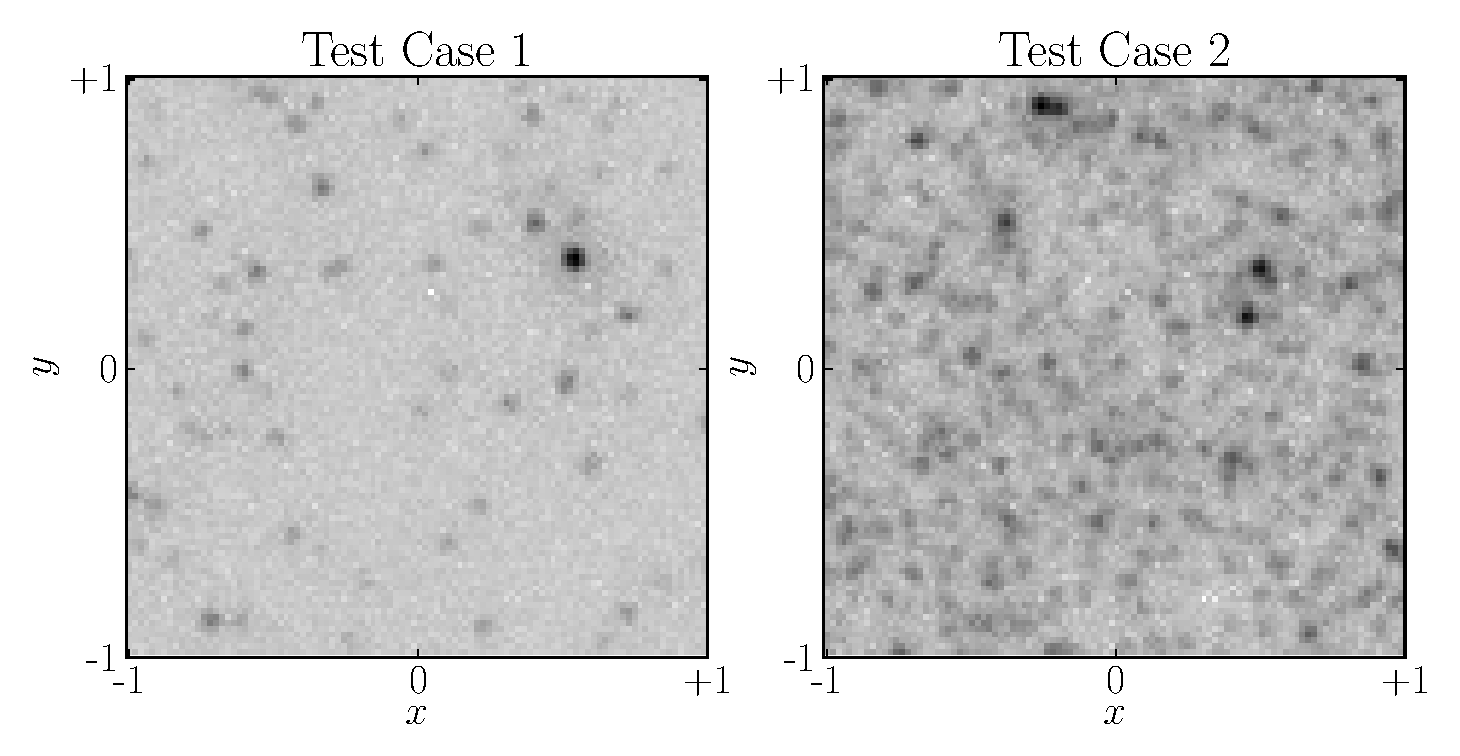
\includegraphics{Figures/test_cases.eps}
\end{figure}

\subsection{Sparse}
Sparse has a giant first-order phase transition. {\bf Nested Sampling is
mandatory!} Show the plot of it

\begin{figure}
\begin{center}
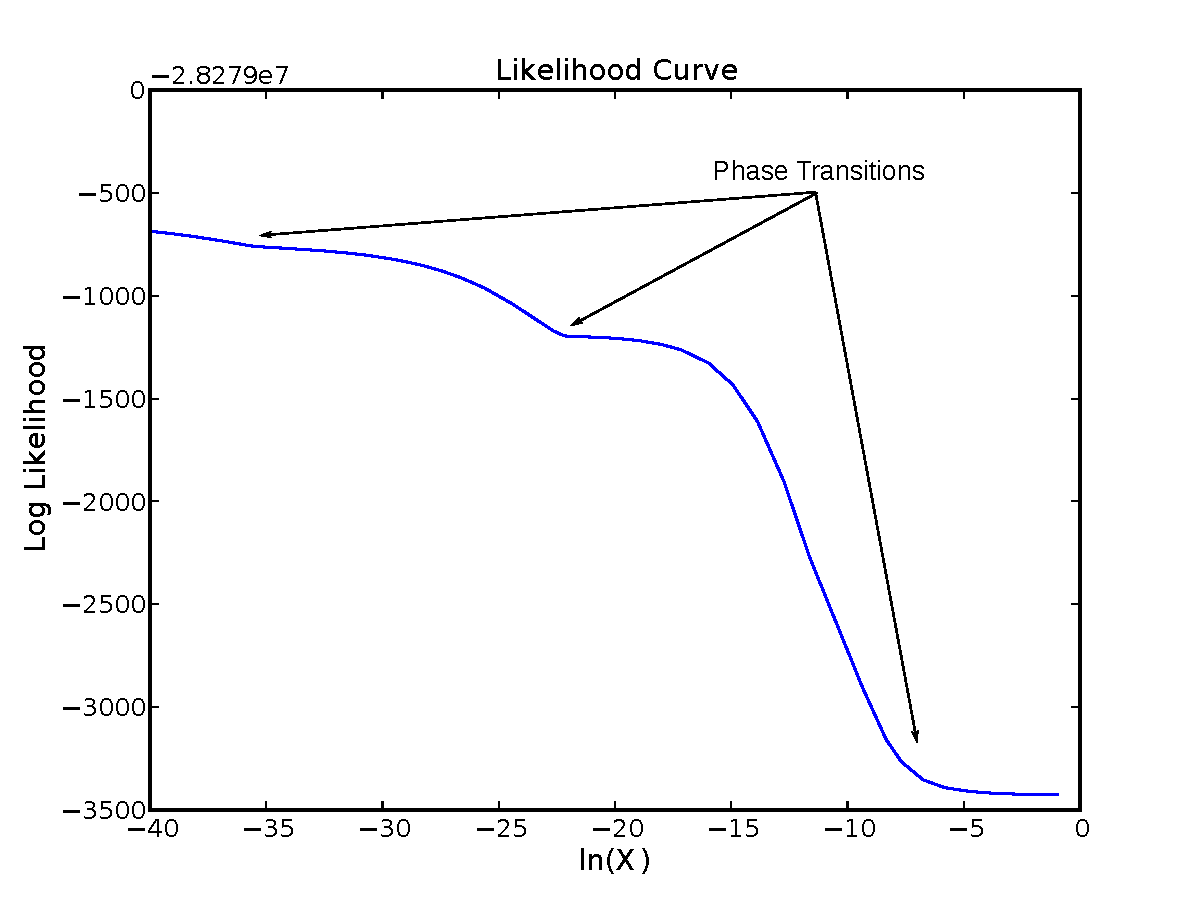
\includegraphics[scale=0.7]{Figures/likelihood.eps}
\end{center}
\end{figure}

\subsection{Cluster}
Was generated from non-uniform spatial distribution (obviously) but modelled
with a uniform one.

\subsection{Crowded}
Crowded is slow if the data have high S/N. Something like $e^5000$ compressions
are needed. Can do NS and not worry about equilibration if you are willing to
make a guess about the logXs of the levels.

\subsection{Toy Model}
For the first implementation I wrote at NYU, I used the following model and
priors:
\begin{itemize}
\item $N \sim \textnormal{Uniform}(0, 1, 2, ..., 1000)$ \\
\item The parameters of the spatial
distribution: $\alpha = \left\{x_c, y_c, \sigma\right\}$ \\
\item The spatial distribution: $p(x_i, y_i | \alpha)\sim\mathcal{N}\left(
\texttt{mean}=(x_c, y_c), \texttt{covariance}=
\left(\begin{array}{cc}\sigma^2 & 0 \\ 0 & \sigma^2\end{array}\right)\right)$ \\
\item Prior on $\alpha$: Uniform within image for $(x_c, y_c)$, logUniform for
$\sigma$ with max value $\sim$ image size.
\item The luminosity function: $p(f_i | \beta) \sim
\textnormal{Exponential}\left(\texttt{mean}=\beta\right)$ \\
\item Prior on $\beta$: logUniform with generous bounds.
\end{itemize}


\section{MCMC Implementation}
\subsection{Current}
I am using Diffusive Nested Sampling \citep{dnest}, which is really just
Metropolis-Hastings but targeting a fancy distribution instead of the actual
posterior, and then assigning importance weights when you want the posterior.
Nested Sampling is good because it is invariant under monotonic transformations
of the likelihood function. i.e. the exploration only depends on things like
whether one point is better than another, and not on how much better it is.

\section{A More Realistic Model}
\citep{2008ApJ...682..874K}


\section{Acknowledgements}
BJB would like to thank his teaching mentor Dr Wayne Stewart.
Marshall, Lang, ...


\appendix
\section{Pixel Convolved PSF}
Consider a ``true image'' $f_0(x, y)$ with infinite resolution. We now model how
this image gives rise to the observed data. First, it is convolved with a
PSF $g(\delta_x, \delta_y)$ (assumed normalized to 1) to give the blurred image:
\begin{eqnarray}
f_{\rm{blurred}}(x, y) &=& \iint f_0(x-\delta_x, y-\delta_y)
g(\delta_x, \delta_y) \, d\delta_x \, d\delta_y \label{blur}
\end{eqnarray}
Then, we observe the blurred image with a certain pixellation. Consider a pixel.
The true flux $F$ within the pixel is:
\begin{eqnarray}
F &=& \iint_{\rm pixel} f_{\rm blurred}(x, y) \,dx'\,dy'\\
&=& \iint f_{\rm blurred}(x, y)\mathbbm{1}\left[(x,y) \in \textnormal{pixel}
\right] \,dx\,dy \label{pixel}
\end{eqnarray}
Now consider $F$ as a function of the central location $(x_c, y_c)$ of the
pixel.




\subsubsection{Proposal Distributions}

\begin{table}
\begin{center}
\begin{tabular}{c|c|c}
Parameter & Proposal & Notes\\
\hline
$N$ & $N \to N + \delta_N$ & Generate $\delta_N$ new stars from prior given
$(\alpha, \beta)$\\
$N$ & $N \to N - \delta_N$ & Remove $\delta_N$ stars at random\\
$\alpha$ & $\alpha \to \alpha + \delta_\alpha$ & Move stars along with $\alpha$
\\
$\alpha$ & $\alpha \to \alpha + \delta_\alpha$ & Stars fixed, use logHastings
factor \\
$\beta$ & $\beta \to \beta + \delta_\beta$ & Move stars' fluxes along with
$\beta$\\
$\beta$ & $\beta \to \beta + \delta_\beta$ & Stars' fluxes fixed, use
logHastings factor \\
$(x,y)$ & $(x,y) \to (x,y)+(\delta_x, \delta_y)$ & Can move $>1$ star.
Include prior via logH \\
$f$ & $f \to f + \delta_f$ & Can move $>1$ stars' fluxes. Include prior
via logH
\end{tabular}
\end{center}
\caption{All $\delta$ parameters are drawn from multi-scale distibutions such
that the largest steps are of order the prior width, and the smallest steps
are of order $10^{-6}$ times the prior width.\label{proposals}}
\end{table}

See Table~\ref{proposals} for a list of current proposal distributions.




%\subsection{Future Possibilities}
%{\bf Hogg}: {\it I think this problem is important enough and general enough
%that we should spend some time working on some ideas there.  If we can sample
%over image explanations, our powers in astronomy will be awesome
%beyond our wildest imaginings.}

%\subsection{Genetic Moves}
%Here I will sketch some ideas...




\begin{thebibliography}{99}
\bibitem[Bertin and 
Arnouts(1996)]{sextractor} Bertin, E., Arnouts, S.\ 1996.\ SExtractor: Software for source extraction.\ Astronomy and Astrophysics Supplement Series 117, 393-404.

\bibitem[\protect\citeauthoryear{Brewer, P{\'a}rtay, 
\& Cs{\'a}nyi}{2011}]{dnest} Brewer B.~J., P{\'a}rtay L.~B.,
Cs{\'a}nyi G., 2011, Statistics and Computing, 21, 4, 649-656. arXiv:0912.2380

\bibitem[Caticha(2009)]{caticha} Caticha, A.\ 2009.\ 
Quantifying Rational Belief.\ American Institute of Physics Conference 
Series 1193, 60-68. 

\bibitem[Cox(1946)]{cox} Cox, R.~T., 1946, Probability, Frequency, and Reasonable Expectation. 1946. American Journal of Physics 14 14, 1-13.

\bibitem[Feroz et al.(2011)]{2011MNRAS.415.3462F} Feroz, F., Balan, S.~T., 
Hobson, M.~P.\ 2011.\ Detecting extrasolar planets from stellar radial 
velocities using Bayesian evidence.\ Monthly Notices of the Royal 
Astronomical Society 415, 3462-3472. 

\bibitem[\protect\citeauthoryear{Green}{1995}]{rjmcmc}
Green, P.~J., 1995, Reversible Jump Markov Chain Monte Carlo Computation and Bayesian Model Determination, Biometrika 82 (4): 711–732.

\bibitem[Jaynes(2003)]{jaynes} Jaynes, E.~T., 2003, Probability Theory: The
Logic of Science, ISBN 0521592712, Cambridge University Press, June 2003.

\bibitem[Kelly et al.(2008)]{2008ApJ...682..874K} Kelly, B.~C., Fan, X., 
\& Vestergaard, M.\ 2008, ApJ, 682, 874 

\bibitem[Mackay(2003)]{mackay} Mackay, D.~J.~C., 2003, Information Theory,
Inference and Learning Algorithms, Cambridge University Press, UK.

\bibitem[\protect\citeauthoryear{Skilling}{1998}]{massinf} 
Skilling J., 1998, Massive Inference and Maximum Entropy, in Maximum Entropy 
and Bayesian Methods, Kluwer Academic Publishers, Dordrecht/Boston/London p.14
\end{thebibliography}

\end{document}

